% TVEIT2025 calibration guide: how to calibrate the Tveit-Ottosen fatigue model for your own material.
% Compile with pdflatex (twice, for the references). Figures are in figures/ (PDF, vector), drawn by
% make_figures.py from the calibrations of the repository.
\documentclass[11pt,a4paper]{article}

\usepackage[margin=25mm]{geometry}
\usepackage[T1]{fontenc}
\usepackage{lmodern}
\usepackage{amsmath,amssymb}
\usepackage{booktabs}
\usepackage{tabularx}
\usepackage{array}
\usepackage{graphicx}
\usepackage{placeins}
\usepackage[dvipsnames]{xcolor}
\usepackage{enumitem}
\usepackage[font=small,labelfont=bf]{caption}
\usepackage{tcolorbox}
\usepackage[colorlinks=true,linkcolor=NavyBlue,citecolor=NavyBlue,urlcolor=NavyBlue]{hyperref}


\graphicspath{{figures/}}
\setlist{itemsep=2pt,topsep=4pt}
\setlength{\parskip}{4pt}
\setlength{\parindent}{0pt}

% Notation
\newcommand{\sigm}{\sigma_{-1}}
\newcommand{\taum}{\tau_{-1}}
\newcommand{\Su}{S_u}
\newcommand{\Emin}{E_{\min}}
\newcommand{\dec}{\,\text{decade}}
\newcommand{\code}[1]{\texttt{#1}}

% Boxes: rule = a fixed choice of this guide; pitfall = a known trap; lesson = what an example teaches
\newtcolorbox{rulebox}[1][]{colback=gray!7,colframe=gray!55,boxrule=0.5pt,arc=1pt,left=5pt,right=5pt,top=3pt,
  bottom=3pt,fonttitle=\bfseries\small,title=Rule#1}
\newtcolorbox{pitfall}[1][]{colback=orange!6,colframe=orange!75!black,boxrule=0.5pt,arc=1pt,left=5pt,right=5pt,
  top=3pt,bottom=3pt,fonttitle=\bfseries\small,title=Pitfall#1}
\newtcolorbox{lesson}[1][]{colback=NavyBlue!5,colframe=NavyBlue!70,boxrule=0.5pt,arc=1pt,left=5pt,right=5pt,
  top=3pt,bottom=3pt,fonttitle=\bfseries\small,title=What this example shows#1}

\title{Calibrating the Tveit--Ottosen fatigue model (TVEIT2025)\\[4pt]
  \large A step-by-step guide with worked examples}
\author{A.~A.~Akay\\ \small FABER WG4.3, \texttt{multifat}}
\date{17 November 2026}

\begin{document}
\maketitle

%=====================================================================================================================
\section{About this guide}
%=====================================================================================================================
This guide explains how to obtain the six constants of the TVEIT2025 fatigue model for a new material from ordinary
fatigue test data. It follows the calibration procedure of Tveit, Ottosen, Erduran and Reyes~\cite{tveit2025}.
Where the article leaves a choice open (which tests to use, or which of several equally good fits to keep), this
guide gives a fixed rule, so that two users with the same data obtain the same constants. Such rules are shown in
grey boxes; known traps are shown in orange boxes.

\texttt{multifat} carries out these steps itself: without supplied constants, \code{multifat-pipeline} calibrates
TVEIT2025 on any fatigue-life workbook, records how, and states how far the result can be trusted
(Section~\ref{sec:confidence}). This guide explains what it does, what data it needs and how to read its result.

The calibration has six steps:

\begin{table}[htbp]
\centering
\caption{Overview of the parameter identification and
model validation procedure.}
\label{tab:calibration_procedure}

\renewcommand{\arraystretch}{1.35}
\setlength{\tabcolsep}{8pt}

\begin{tabularx}{\textwidth}{
    @{}
    >{\centering\arraybackslash}p{0.08\textwidth}
    >{\raggedright\arraybackslash}p{0.29\textwidth}
    >{\raggedright\arraybackslash}X
    @{}
}
\toprule
\textbf{Step} &
\textbf{Determines} &
\textbf{Method / Data source} \\
\midrule

1
& $\sigm$, $\taum$, $\lambda$
& Fully reversed ($R=-1$) axial and torsional
fatigue limits. \\

\addlinespace[3pt]

2
& $A$
& Fatigue limit at a tensile mean stress;
alternatively, a hand-entered value, or the FKM or Goodman estimate. \\

\addlinespace[3pt]

3
& ---
& Selection of three axial fatigue failures
($R=-1$) using a predefined, fixed rule. \\

\addlinespace[3pt]

4
& $C$, $K$, $L$ (equivalent sets)
& Least-squares fit to the three fatigue lives
(Eq.~\ref{eq:E}), profiled over a fixed grid of $C$. \\

\addlinespace[3pt]

5
& $C$, $K$, $L$ (final set)
& Two acceptance checks, and selection
of the lowest-error set that passes them. \\

\midrule

6
& ---
& \textbf{Validation:} evaluate residuals,
predict independent experimental results,
and document model performance. \\

\bottomrule
\end{tabularx}
\end{table}
Section~\ref{sec:examples} applies the steps to six workbooks of the \texttt{multifat} database: Al7075-T6,
two batches each of Ti6Al4V and 42CrMo4, and Al7075-T651.

%=====================================================================================================================
\section{The model in brief}\label{sec:model}
%=====================================================================================================================
\FloatBarrier

For a stress history $\boldsymbol{\sigma}(t)$, let $\mathbf{s}$ be the stress deviator and $\boldsymbol{\alpha}$ a
deviatoric back-stress, with $\hat{\mathbf{s}}=\mathbf{s}-\boldsymbol{\alpha}$. The model uses an effective stress
of the reduced deviator,
\begin{equation}
  \sigma_e = \sqrt{3J_2} - \lambda\left(1-\frac{27}{4}\,\frac{J_3^2}{J_2^3}\right),
  \qquad \lambda=\sqrt{3}\,\taum-\sigm ,
  \label{eq:se}
\end{equation}
where $J_2$ and $J_3$ are the invariants of $\hat{\mathbf{s}}$, and the endurance function
\begin{equation}
  \beta = \frac{\sigma_e + A\,I_1 - \sigm}{\sigm}, \qquad I_1=\operatorname{tr}\boldsymbol{\sigma}.
  \label{eq:beta}
\end{equation}
Nothing happens while $\beta<0$ (inside the endurance surface). While $\beta\ge 0$ and $\dot\beta>0$, the back-stress
follows the stress and damage grows:
\begin{equation}
  \dot{\boldsymbol{\alpha}} = C\,\dot\beta\,\hat{\mathbf{s}}, \qquad
  \dot D = K\,e^{L\beta}\,\dot\beta .
  \label{eq:evol}
\end{equation}
Failure occurs at $D=1$. If the back-stress settles so that the stress no longer leaves the endurance surface
(shakedown), damage stops and the life is infinite.

\begin{table}[htbp]
\centering
\caption{Model parameters, physical interpretation,
and identification procedure.}
\label{tab:model_parameters}

\renewcommand{\arraystretch}{1.35}
\setlength{\tabcolsep}{8pt}

\begin{tabularx}{\textwidth}{
    @{}
    >{\centering\arraybackslash}p{0.13\textwidth}
    >{\centering\arraybackslash}p{0.10\textwidth}
    >{\raggedright\arraybackslash}X
    >{\centering\arraybackslash}p{0.19\textwidth}
    @{}
}
\toprule
\textbf{Parameter} &
\textbf{Unit} &
\textbf{Physical interpretation} &
\textbf{Identified in} \\
\midrule

$\sigm$
& MPa
& Axial fatigue limit under fully reversed
loading ($R=-1$).
& Step 1 \\

\addlinespace[3pt]

$\taum$
& MPa
& Torsional fatigue limit under fully reversed
loading ($R=-1$); contributes through $\lambda$.
& Step 1 \\

\addlinespace[3pt]

$A$
& ---
& Sensitivity to hydrostatic stress
(mean-stress effects).
& Step 2 \\

\midrule

$C$
& ---
& Controls the rate of back-stress evolution.
& Steps 4--5 \\

\addlinespace[3pt]

$K$
& ---
& Scaling factor governing the damage
accumulation rate.
& Steps 4--5 \\

\addlinespace[3pt]

$L$
& ---
& Damage-rate exponent governing the
sensitivity of damage evolution to $\beta$.
& Steps 4--5 \\

\bottomrule
\end{tabularx}
\end{table}

Three properties of the model shape the calibration:
\begin{enumerate}[label=(P\arabic*)]
\item \textbf{The uniaxial endurance limit is a straight Haigh line,}
  \begin{equation}
    \sigma_a + A\,\sigma_m = \sigm .
    \label{eq:haigh}
  \end{equation}
  $\sigm$ is its intercept at $\sigma_m=0$ and $A$ its (negative) slope. Below the line the steady cycle produces no
  damage.
\item \textbf{Uniaxial $R=-1$ S--N data do not identify $C$.} Many combinations of $C$, $K$ and $L$ give practically
  the same uniaxial S--N curve; $C$ can vary over four decades or more (Step~5).
\item \textbf{In torsion $I_1=0$, and a mean shear stress is absorbed by the back-stress.} It does not lower the
  torsion endurance limit and acts only through the damage of the first cycles, whose size depends on $C$ and $L$.
\end{enumerate}

\FloatBarrier
%=====================================================================================================================
\section{The data you need}
%=====================================================================================================================
\begin{table}[h]
\centering
\caption{Experimental data required for parameter calibration
and model validation.}
\label{tab:required_data}

\renewcommand{\arraystretch}{1.35}
\setlength{\tabcolsep}{8pt}

\begin{tabularx}{\textwidth}{
    @{}
    >{\raggedright\arraybackslash}p{0.39\textwidth}
    >{\centering\arraybackslash}p{0.12\textwidth}
    >{\raggedright\arraybackslash}X
    @{}
}
\toprule
\textbf{Experimental data} &
\textbf{Step} &
\textbf{Remarks} \\
\midrule

Axial fatigue limit, $\sigm$ ($R=-1$)
& 1
& Same material batch and laboratory as the S--N tests, with the life at which it is defined. \\

\addlinespace[3pt]

Torsional fatigue limit, $\taum$ ($R=-1$)
& 1
& Same requirements as above. \\

\addlinespace[3pt]

Fatigue limit at a tensile mean stress
(e.g., axial $R=0$ or $R=0.1$)
& 2
& Preferred approach for determining $A$. \\

\addlinespace[3pt]

Ultimate tensile strength, $\Su$
& 2
& Alternative if mean-stress fatigue data are unavailable. \\

\addlinespace[3pt]

Axial fatigue failures ($R=-1$) at
$\geq 3$ stress levels above $\sigm$
& 3--5
& Preferably with replicates and fatigue lives
between $10^4$ and $10^6$ cycles. The source of each test (authors, DOI) is needed to match it to the limits. \\

\midrule

Other fatigue tests (torsional S--N,
mean-stress, and multiaxial loading)
& 6
& \textbf{Validation only.} Not used for
parameter calibration. \\

\bottomrule
\end{tabularx}
\end{table}

In \texttt{multifat}, the limits, $\Su$ and the life at which the limits are defined (\code{Number of Cycles}) are
read from the \code{Summary} sheet of the workbook, and the tests and their sources from its \code{Dataset} sheet.
What a workbook cannot hold (a fatigue limit at a mean stress, a hand-entered $A$, the material type for FKM) goes
in an optional file \code{Calibrations/<material>/TVEIT2025\_inputs.json} (Step~2).

\FloatBarrier
%=====================================================================================================================
\section{The procedure}\label{sec:procedure}
%=====================================================================================================================

\subsection*{Step 1: fatigue limits and $\lambda$}
Take $\sigm$ and $\taum$ from the material data and compute $\lambda=\sqrt3\,\taum-\sigm$.

\begin{rulebox}
Use the limits of the workbook (its fully reversed axial and torsion rows), and calibrate on the tests of the same
source: the same DOI, else the same authors.
\end{rulebox}

\begin{pitfall}
Databases often pool tests from several sources but list one fatigue limit. A limit taken from one source and applied
to another source's tests puts tests on the wrong side of the endurance surface: failures below $\sigm$ are then
predicted to last forever. Check $\sigm$ against the run-outs and the failures near the limit; a censored maximum-likelihood
fit of the limit is one way. \texttt{multifat} lists such failures in the confidence of the calibration
(Section~\ref{sec:confidence}, Example~3).
\end{pitfall}

\begin{pitfall}[: a limit defined at a finite life]
Some materials, such as aluminium alloys, have no true fatigue limit: the limit is the S--N curve at a reference life,
for example $10^6$ cycles. A failure below it after that life agrees with the limit; in the model, however, $\sigm$
is a true threshold, so it predicts an infinite life for that test (Example~4).
\end{pitfall}

\subsection*{Step 2: the mean-stress constant $A$}
\FloatBarrier
By (P1), $A$ is the slope of the Haigh line. Use the first route your data allow (Fig.~\ref{fig:haigh}):
\begin{table}[h]
\centering
\caption{Alternative approaches for identifying the
mean-stress sensitivity parameter $A$, in the order of the article.}
\label{tab:mean_stress_identification}

\renewcommand{\arraystretch}{1.35}
\setlength{\tabcolsep}{8pt}

\begin{tabularx}{\textwidth}{
    @{}
    >{\centering\arraybackslash}p{0.14\textwidth}
    >{\raggedright\arraybackslash}p{0.30\textwidth}
    >{\raggedright\arraybackslash}X
    @{}
}
\toprule
\textbf{Route} &
\textbf{Required data} &
\textbf{Determination of $A$} \\
\midrule

1 (Article)
& Fatigue limit $(\sigma_{m,0},\sigma_{a,0})$
at a tensile mean stress.
& Direct identification using the article's
Eqs.~22--23:
\[
A = \frac{\sigm-\sigma_{a,0}}{\sigma_{m,0}}.
\] \\[-6pt]

\addlinespace[3pt]

2 (Hand-entered)
& A value of $A$ obtained otherwise, with its source.
& For example, mean-stress failures without an established fatigue limit: Eq.~23 then gives only a lower
bound, and $A$ can be chosen to reproduce the life of one mean-stress test, re-fitting $C$, $K$ and $L$
(Steps 4--5) for each trial value of $A$. \\

\midrule

3 (FKM)
& Ultimate tensile strength $\Su$ and the material type.
& FKM mean-stress sensitivity (article's Eq.~26):
\[
A = M_\sigma
  = a_M\frac{\Su}{1000}+b_M.
\]
For steel, $a_M=0.35$ and $b_M=-0.1$,
with $\Su$ in MPa~\cite{fkm}. \\[-6pt]

\addlinespace[3pt]

4 (Goodman)
& Ultimate tensile strength, $\Su$.
& Linear Goodman approximation, which the article uses where FKM gives no values:
\[
A = \frac{\sigm}{\Su}.
\] \\[-6pt]

\bottomrule
\end{tabularx}
\end{table}

\begin{figure}[ht]
  \centering
  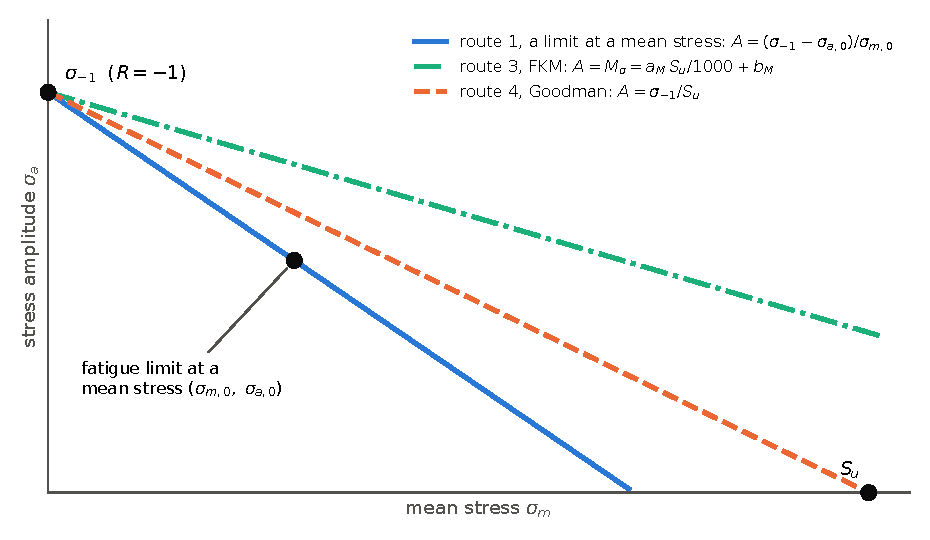
\includegraphics[width=0.82\textwidth]{fig_haigh_routes.pdf}
  \caption{The model's uniaxial endurance limit is the Haigh line $\sigma_a+A\,\sigma_m=\sigm$ (slope $-A$); below it
  the steady cycle produces no damage. The routes to $A$ differ only in how the slope is obtained (schematic).}
  \label{fig:haigh}
\end{figure}

In \texttt{multifat}, routes 1 to 3 are declared in the inputs file; without one, $A$ is the Goodman estimate. For
example (Al7075-T6, route 1):
\begin{verbatim}
  {
   "schema": "multifat/tveit2025-calibration-inputs/2",
   "material_id": "Al7075_T6",
   "mean_stress_fatigue_limit": {"sigma_a": 100.0, "R": 0.1, "source": "..."}
  }
\end{verbatim}
Route 2 is \code{"A": \{"value": ..., "source": ...\}} and route 3 \code{"material\_type": "steel"}; the FKM values
in \texttt{multifat} cover steel only.

\begin{rulebox}
Fix $A$ before Step 4. The $R=-1$ lives depend on $A$ too, because $I_1$ varies within the cycle, so $C$, $K$ and $L$
are conditional on $A$. If $A$ changes, repeat Steps 4--6.
\end{rulebox}

\begin{pitfall}
Routes 3 and 4 depend on the value of $\Su$; record which value you used. For 42CrMo4, two revisions of the same
database give $\Su=987.5$ and $875$~MPa, i.e.\ $A=0.2456$ and $0.2063$ with FKM.
\end{pitfall}

\FloatBarrier
\subsection*{Step 3: three calibration points}
The article calibrates $C$, $K$ and $L$ on three uniaxial S--N points. The rule below makes the choice reproducible.

\begin{rulebox}
\begin{enumerate}[leftmargin=*]
\item Candidates: plain (unnotched) axial $R=-1$ failures of the source of the limits, with $\sigma_a$ strictly
  above $\sigm$.
\item Levels: the distinct stress amplitudes among the candidates.
\item LOW = the lowest level; HIGH = the highest level; MID = the level, other than these two, closest to
  $\sqrt{\text{LOW}\cdot\text{HIGH}}$ on a logarithmic scale.
\item At each chosen level, take the replicate whose $\log N$ is closest to the median $\log N$ of that level. On an
  exact tie, take the first one listed.
\end{enumerate}
\end{rulebox}

\begin{pitfall}
\begin{itemize}[leftmargin=*]
\item A level with a single specimen that disagrees with other data can bend the whole curve (Example~3).
\item Points whose stresses lie within a few per cent of each other carry no S--N trend; the fit then degenerates
  (e.g.\ $L$ ends at its bound, Example~2).
\item $\sigm$ is the asymptote of the model curve. A LOW point just above $\sigm$ is hard to fit exactly; expect a
  residual of a few tenths of a decade there.
\end{itemize}
\end{pitfall}

\FloatBarrier
\subsection*{Step 4: fit $C$, $K$ and $L$}
Minimise the objective of the article (Eq.~25 there),
\begin{equation}
  E(C,K,L) = \sum_{i=1}^{3}\left(1-\frac{\ln N_i}{\ln N_{i,\text{exp}}}\right)^{2},
  \label{eq:E}
\end{equation}
where $N_i$ is the model life of calibration point $i$ from the closed-form steady-cycle uniaxial solution of Ottosen
et al.~\cite{ottosen2008} (with $\sigm$, $\lambda$ and $A$ fixed). If the closed form gives no finite life at a
point, that point gets a penalty (10 in place of the squared term).

\begin{rulebox}
Profile $E$ over $C$: a fixed grid of $C$, 8 values per decade over $[10^{-4},10^{3}]$; at each $C$, $K$ and $L$ are
fitted by a simplex search inside $K\in[10^{-12},10^{-1}]$, $L\in[0.05,50]$. $\Emin$ is the lowest $E$ over the grid,
and the \emph{equivalent sets} are the grid points with $E\le 1.05\,\Emin$. A multi-start search would return an
arbitrary member of this family; the grid returns the same family on every run.
\end{rulebox}

Three parameters and three points do not give an exact fit: with $\sigm$ fixed, the curve has a fixed asymptote and
cannot pass through three arbitrary points. In the examples, $\Emin$ lies between $2.4\times10^{-4}$ and
$7.8\times10^{-3}$, with residuals of up to $0.37\dec$ at single points.

\FloatBarrier
\subsection*{Step 5: choose one set}
\begin{enumerate}[label=(\alph*)]
\item \textbf{Two checks} at each calibration point:
  \begin{itemize}
  \item G1: the closed form has a unique valid solution;
  \item G2: the full transient model (Eqs.~\ref{eq:se}--\ref{eq:evol}, integrated cycle by cycle) and the closed form
    agree within $0.10\dec$ in life.
  \end{itemize}
  G2 matters because the closed form ignores the damage of the first cycles, before the back-stress settles. With a
  slow back-stress (small $C$), these cycles do much of the damage at a high stress: in the examples, the closed form
  overestimates the life at the HIGH point by up to $0.8\dec$ for the slowest sets.
\item \textbf{Choice:} among the equivalent sets, the one with the lowest $E$ that passes both checks.
\end{enumerate}

\begin{pitfall}[: $C$ is not identified by the calibration data]
In five of the six examples, the equivalent sets span more than four decades in $C$, yet give the same uniaxial
S--N curve
(Figs.~\ref{fig:al}--\ref{fig:wang}). The lowest-$E$ choice therefore fixes $C$ by convention, not by data.
$C$ matters where the back-stress dynamics matter: loading with a mean shear stress, and non-proportional loading
such as $90^\circ$ out-of-phase tension--torsion. Report the range of $C$ among the equivalent sets together with the
chosen set. Check G2 can remove the slowest part of the family (Examples 2 and 3), and well-spread points can narrow
it (Example~3).
\end{pitfall}

\FloatBarrier
\subsection*{Step 6: check and record}
\begin{itemize}
\item Report the residuals $\log_{10}(N_\text{pred}/N_\text{exp})$ at the three points, from both the closed form and
  the transient model.
\item Predict every other test with the transient model, never with the closed form.
\item Never change the constants because of the validation results. A new calibration starts again at Step~1, with its
  reasons written down before the new results are seen.
\item Record the six constants with their provenance: data source, route to $A$, the three points, the range of
  $C$ among the equivalent sets, and the confidence (Section~\ref{sec:confidence}).
\end{itemize}
\texttt{multifat} writes all of this to a record, archived with the run and committed for the materials of the
database under \code{Calibrations/<material>/}; the three calibration tests become design rows. An identical
calibration (the same workbook, overlay, inputs file, procedure version and implementation) is reused instead of
repeated. A
\code{--constants} file takes precedence over the calibration, and \code{--no-calibrate} turns it off. For
Al7075-T6:
\begin{verbatim}
  "params": {
      "Sigm1_TVEIT": 143.8,
      "Taum1_TVEIT": 100.9,
      "A_TVEIT": 0.35836363636363644,
      "C_TVEIT": 0.0001,
      "K_TVEIT": 3.2873746239497344e-06,
      "L_TVEIT": 2.9746140900192004,
      ...
  }
\end{verbatim}

%=====================================================================================================================
\section{How far can the calibration be trusted?}\label{sec:confidence}
%=====================================================================================================================
Each calibration lists what weakens it. Every \emph{finding} says what was found, why it matters and what data would
remove it, and it is either \emph{major}, when the calibration probably misrepresents the material (inconsistent data,
a degenerate fit), or \emph{minor}, for a known limitation or an estimate the authors themselves use. The confidence
level follows: \textbf{high} without findings, \textbf{medium} with minor findings only, \textbf{low} with a major one.
The findings use only the calibration inputs and the fit, never the predictions of other tests.

\begin{table}[htbp]
\centering
\caption{Findings of the calibration confidence.}
\label{tab:findings}
\small
\renewcommand{\arraystretch}{1.25}
\begin{tabularx}{\textwidth}{
    @{}
    >{\raggedright\arraybackslash}p{0.30\textwidth}
    >{\centering\arraybackslash}p{0.08\textwidth}
    >{\raggedright\arraybackslash}X
    @{}
}
\toprule
\textbf{Finding} & \textbf{Severity} & \textbf{Meaning, and what removes it} \\
\midrule
\code{failures\_below\_limit} & major & Axial $R=-1$ failures below $\sigm$ before its reference life: the data
contradict the limit. Check $\sigm$ against the failures and run-outs of the source. \\
\code{late\_failures\_below\_limit} & minor & Failures below $\sigm$ after its reference life: they agree with a limit
defined at that life, but the model predicts an infinite life for them. A limit at a longer reference life. \\
\code{runouts\_above\_limit} & minor & Axial $R=-1$ run-outs above $\sigm$: the limit may be conservative. \\
\code{limit\_source\_differs} & major & No test of the source of the limits. Use the limits of the source of the
tests. \\
\code{limit\_other\_publication} & minor & Limits from another publication of the same authors. Confirm the same
batch. \\
\code{points\_mixed\_sources} & major & Calibration points from several sources. Calibrate on one source. \\
\code{point\_not\_R\_minus\_1} & major & A calibration point with a mean stress. Use $R=-1$ failures. \\
\code{A\_estimated} & minor & $A$ from FKM or Goodman. A fatigue limit at a tensile mean stress. \\
\code{A\_supplied} & minor & $A$ entered by hand. A fatigue limit at a tensile mean stress. \\
\code{material\_type\_for\_FKM} & minor & Goodman because no material type is declared. Declare it. \\
\code{narrow\_stress\_range} & major & HIGH/LOW below 1.10: the points carry no S--N trend. Failures over a wider
stress range. \\
\code{low\_point\_near\_limit} & minor & LOW within 5\,\% of $\sigm$. A LOW level further above the limit. \\
\code{single\_specimen\_level} & minor & A chosen level with one specimen. More replicates. \\
\code{poor\_fit} & minor & A point missed by more than $0.3\dec$. Check the limit and the points. \\
\code{constant\_at\_bound} & major & $K$ or $L$ on its search bound, or $C$ where the equivalent sets pin it. More
informative tests. \\
\code{C\_not\_identified} & minor & $C$ varies over more than one decade among the equivalent sets. A test with a mean
shear stress or $90^\circ$ out-of-phase tension--torsion. \\
\code{point\_at\_block\_limit} & minor & The transient integration of a calibration point reached its block limit, so
its life is extrapolated. A larger block limit. \\
\bottomrule
\end{tabularx}
\end{table}

\FloatBarrier
%=====================================================================================================================
\section{Worked examples}\label{sec:examples}
%=====================================================================================================================
Each example follows Steps 1--6, with the numbers of the \texttt{multifat} calibration. Lives are cycles to failure;
residuals are $\log_{10}(N_\text{pred}/N_\text{exp})$ given as closed form / transient. The figures show the
closed-form curves of all equivalent sets; check G2 is not applied to them.

%---------------------------------------------------------------------------------------------------------------------
\subsection*{Example 1: Al7075-T6 --- everything from one source}
Data: Pedranz et al., \texttt{Al7075\_T6.xlsx}; 11 axial $R=-1$ failures and 2 run-outs.
\begin{description}[leftmargin=0pt,font=\normalfont\bfseries]
\item[Step 1.] $\sigm=143.8$~MPa, $\taum=100.9$~MPa, defined at $5\times10^6$ cycles, so
  $\lambda=\sqrt3\cdot100.9-143.8=31.0$~MPa.
\item[Step 2.] Route 1. The axial $R=0.1$ fatigue limit is $\sigma_{a,0}=100$~MPa (inputs file), at
  $\sigma_{m,0}=\sigma_{a,0}(1+R)/(1-R)=122.2$~MPa. Hence $A=(143.8-100)/122.2=0.358$.
\item[Step 3.] Levels 150, 170, 190 and 230~MPa (2, 3, 3 and 3 specimens). MID: $\sqrt{150\cdot230}=185.7$, so
  190~MPa.
  \begin{center}
  \begin{tabular}{@{}l l r r r@{}}
  \toprule
  Point & Specimen & $\sigma_a$ [MPa] & $N_\text{exp}$ & Residual \\
  \midrule
  LOW & Plain\_axial\_8 & 150.0 & 2\,807\,604 & $+0.07$ / $+0.06$ \\
  MID & Plain\_axial\_1 & 190.0 & 322\,262 & $-0.09$ / $-0.10$ \\
  HIGH & Plain\_axial\_12 & 230.0 & 73\,200 & $+0.03$ / $0.00$ \\
  \bottomrule
  \end{tabular}
  \end{center}
\item[Steps 4--5.] $\Emin=4.02\times10^{-4}$. 34 equivalent sets, $C$ from $10^{-4}$ to 3.16. The lowest-$E$ set
  passes G1 and G2: $C=10^{-4}$ (the lower end of the grid), $K=3.29\times10^{-6}$, $L=2.97$ (Fig.~\ref{fig:al}).
\item[Confidence.] Medium, three minor findings: $C$ not identified; the LOW point lies within 4.3\,\% of $\sigm$;
  one run-out (150~MPa, $5\times10^6$ cycles) lies above $\sigm$.
\end{description}

\begin{figure}[ht]
  \centering
  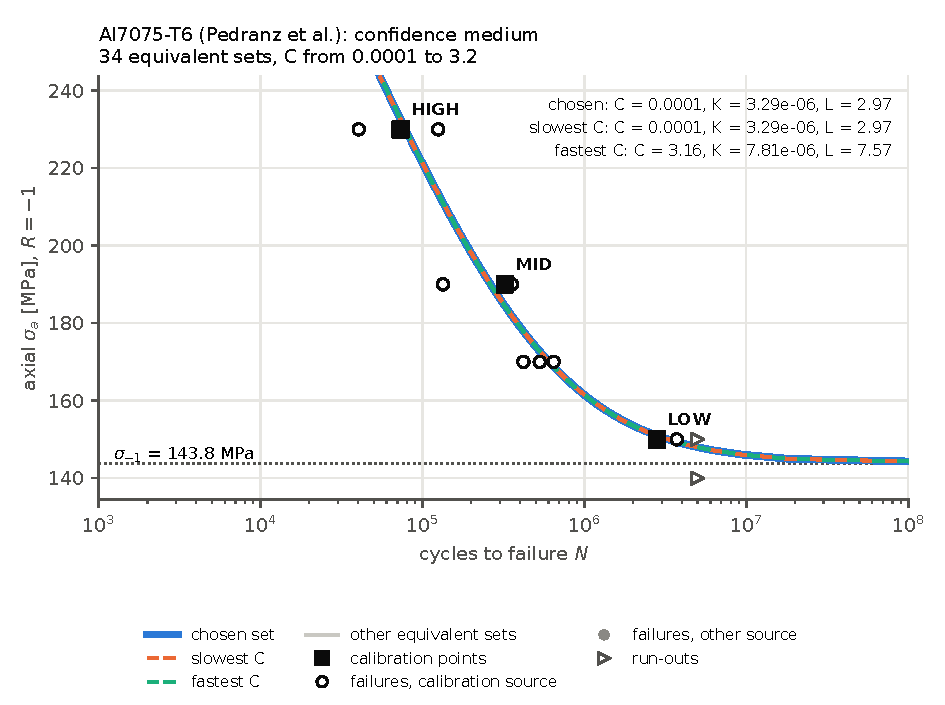
\includegraphics[width=0.85\textwidth]{fig_example_Al7075T6.pdf}
  \caption{Example 1, Al7075-T6. Closed-form uniaxial curves of all 34 equivalent sets: they coincide, although $C$
  changes by more than four decades.}
  \label{fig:al}
\end{figure}

\begin{lesson}
The cleanest case: limits, $A$ and the three points all come from one source, and $A$ follows the article's route.
Even so, the confidence is medium: the uniaxial data cannot fix $C$, the LOW level is close to the limit, and a
run-out above the limit suggests that the limit may be conservative.
\end{lesson}

\FloatBarrier
%---------------------------------------------------------------------------------------------------------------------
\subsection*{Example 2: Ti6Al4V --- $A$ from Goodman, and points too close together}
Two batches of the same alloy, each in its own workbook with its own limits: Berto et al.
(\texttt{15\_Ti6Al4V\_Berto.xlsx}) and Meneghetti et al. (\texttt{1\_Ti6Al4V\_Meneghetti.xlsx}). No fatigue limit
at a mean stress exists, and FKM gives no values for titanium alloys, so both use route 4 (Goodman); the inputs file
declares the material type (Fig.~\ref{fig:ti}).

\begin{center}
\begin{tabular}{@{}l l l@{}}
\toprule
 & Berto et al. & Meneghetti et al. \\
\midrule
$\sigm$ / $\taum$ [MPa] & 475.74 / 388.25 & 500 / 422.5 \\
$\lambda$ [MPa] & 196.7 & 231.8 \\
$A$ (route 4, Goodman) & $475.74/978=0.4864$ & $500/980=0.5102$ \\
Candidates & 9 failures, 510.8 to 822.5~MPa & 6 failures, 523.2 to 550.5~MPa \\
$\Emin$ & $6.50\times10^{-4}$ & $3.63\times10^{-3}$ \\
Equivalent sets & 29, $C$ from $10^{-4}$ to 3.16 & 37, $C$ from $10^{-4}$ to 3.16 \\
Chosen $C$ / $K$ / $L$ & $5.62\times10^{-4}$ / $7.70\times10^{-6}$ / 3.61 & 1.33 / $1.71\times10^{-4}$ / 0.05 \\
Confidence & medium & low \\
\bottomrule
\end{tabular}
\end{center}

\begin{description}[leftmargin=0pt,font=\normalfont\bfseries]
\item[Berto et al.] Eight levels, almost all with a single specimen. MID: $\sqrt{510.8\cdot822.5}=648.1$, closest
  level 613.5~MPa.
  \begin{center}
  \begin{tabular}{@{}l l r r r@{}}
  \toprule
  Point & Specimen & $\sigma_a$ [MPa] & $N_\text{exp}$ & Residual \\
  \midrule
  LOW & Axial\_Plain\_8 & 510.8 & 602\,215 & $+0.09$ / $+0.07$ \\
  MID & Axial\_Plain\_4 & 613.5 & 138\,140 & $-0.10$ / $-0.12$ \\
  HIGH & Axial\_Plain\_1 & 822.5 & 11\,031 & $+0.02$ / $-0.06$ \\
  \bottomrule
  \end{tabular}
  \end{center}
  Check G2 rejects the six slowest equivalent sets ($C$ from $10^{-4}$ to $4.2\times10^{-4}$): at the HIGH point their
  transient life is up to $0.5\dec$ shorter than the closed form. Confidence medium: $A$ estimated, $C$ not
  identified, single specimens at the three levels.
\item[Meneghetti et al.] Levels 523.2, 527.0, 534.7 and 550.5~MPa; MID: $\sqrt{523.2\cdot550.5}=536.7$, so
  534.7~MPa. The three points span 5.2\,\%, and the HIGH point lives longer than the MID one:
  \begin{center}
  \begin{tabular}{@{}l r r r@{}}
  \toprule
  Point & $\sigma_a$ [MPa] & $N_\text{exp}$ & Residual \\
  \midrule
  LOW & 523.2 & 85\,645 & $+0.04$ / $+0.03$ \\
  MID & 534.7 & 42\,965 & $+0.17$ / $+0.16$ \\
  HIGH & 550.5 & 74\,236 & $-0.23$ / $-0.24$ \\
  \bottomrule
  \end{tabular}
  \end{center}
  $L$ ends on its lower bound, 0.05, in every equivalent set. Confidence low, with two major findings ($L$ on its
  bound, stress range too narrow) and four minor ones ($A$ estimated, $C$ not identified, the LOW point within
  4.6\,\% of $\sigm$, single specimens).
\end{description}

\begin{figure}[ht]
  \centering
  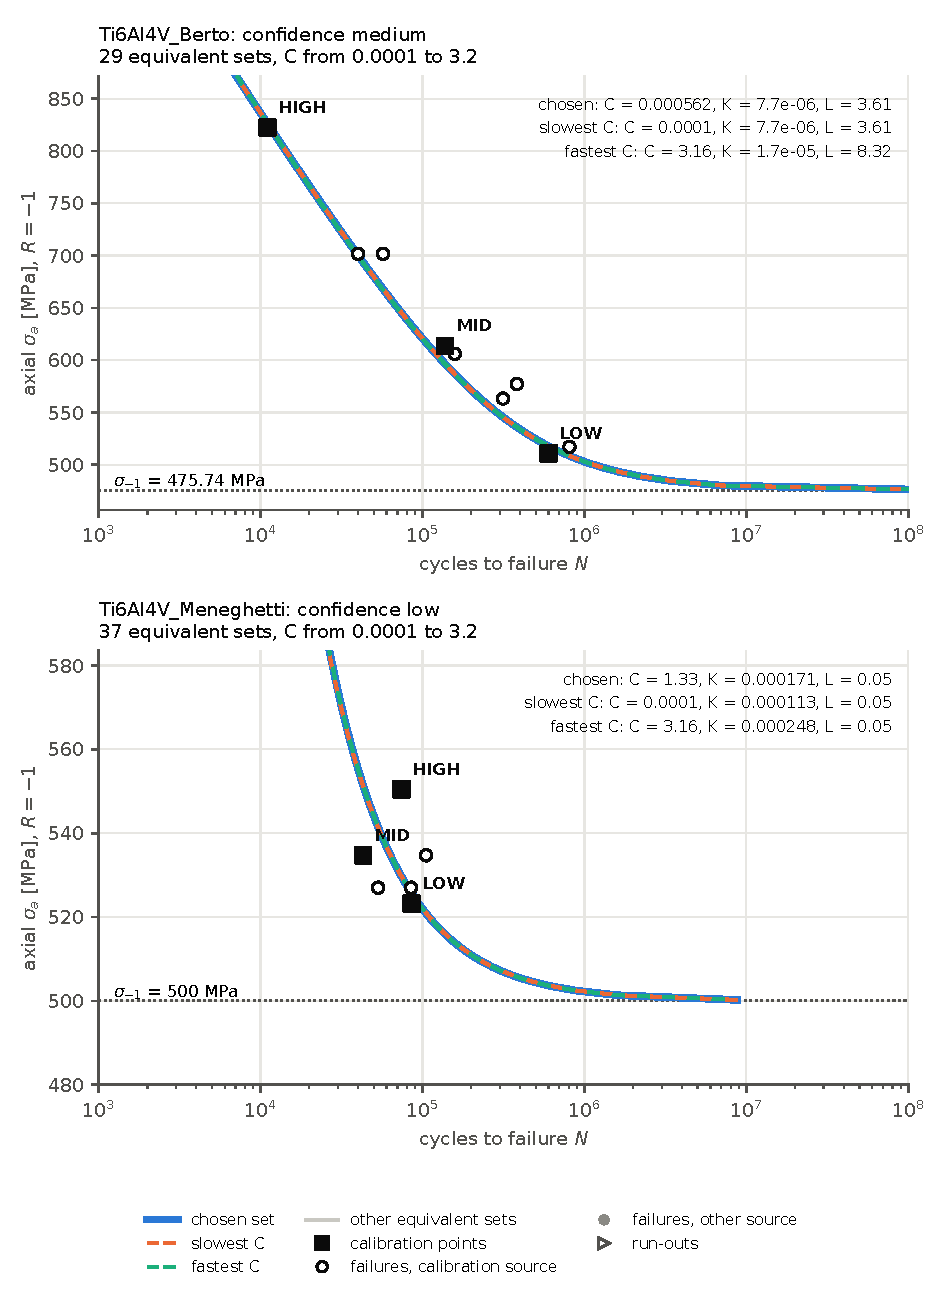
\includegraphics[width=0.85\textwidth]{fig_example_Ti6Al4V.pdf}
  \caption{Example 2, Ti6Al4V. Top: Berto et al., three well-separated points. Bottom: Meneghetti et al., all
  failures within 5\,\% in stress; the fit cannot follow the points and $L$ sits on its bound.}
  \label{fig:ti}
\end{figure}

\begin{lesson}
$A$ from Goodman when no mean-stress limit is available and FKM gives no values. Check G2 removes the slowest
back-stresses. And three points at almost the same stress carry no S--N trend: the fit degenerates, and the low
confidence says so, with what to add (failures over a wider stress range).
\end{lesson}

\FloatBarrier
%---------------------------------------------------------------------------------------------------------------------
\subsection*{Example 3: 42CrMo4 --- $A$ from FKM, a limit contradicted by another source, and $C$ narrowed}
Two batches of 42CrMo4 steel, both with $A$ from route 3 (FKM, steel; the inputs file declares the material type),
Fig.~\ref{fig:cr}.
\begin{description}[leftmargin=0pt,font=\normalfont\bfseries]
\item[\texttt{6\_42CrMo4\_Santus.xlsx}.] The workbook holds the tests of Benedetti et al.\ and of Santus et al.; the
  limits are those of Benedetti et al., $\sigm=433$~MPa and $\taum=344$~MPa at $2\times10^6$ cycles
  ($\lambda=162.8$~MPa), so the calibration uses Benedetti's 10 failures. $A=0.35\cdot875/1000-0.1=0.2063$.
  Levels 450, 500, 550 and 600~MPa (3, 3, 2 and 1 specimens); MID: $\sqrt{450\cdot600}=519.6$, so 500~MPa.
  \begin{center}
  \begin{tabular}{@{}l l r r r@{}}
  \toprule
  Point & Specimen & $\sigma_a$ [MPa] & $N_\text{exp}$ & Residual \\
  \midrule
  LOW & Plain\_axial\_24 & 450.0 & 274\,825 & $+0.29$ / $+0.28$ \\
  MID & Plain\_axial\_20 & 500.0 & 147\,470 & $-0.36$ / $-0.37$ \\
  HIGH & Plain\_axial\_31 & 600.0 & 3\,620 & $+0.05$ / $-0.05$ \\
  \bottomrule
  \end{tabular}
  \end{center}
  $\Emin=7.82\times10^{-3}$; 39 equivalent sets, $C$ from $10^{-4}$ to 5.62 and $L$ from 10.4 to 39. Check G2
  rejects the ten slowest (up to $0.8\dec$ at the HIGH point). Chosen: $C=1.78\times10^{-3}$,
  $K=1.90\times10^{-5}$, $L=10.4$.

  Confidence low. The major finding: 12 axial $R=-1$ failures lie below $\sigm=433$~MPa and failed before
  $2\times10^6$ cycles (lowest 361.1~MPa); 11 of them are of Santus et al., one (425~MPa) of Benedetti et al. Minor
  findings: one more failure below $\sigm$ after $2\times10^6$ cycles, $A$ estimated, $C$ not identified, the LOW
  point within 3.9\,\% of $\sigm$, the MID point missed by $0.37\dec$, and a single specimen at the HIGH level.
\item[\texttt{14\_42CrMo4\_Reis.xlsx}.] Tests of Anes et al., with the limits of another publication of the same
  authors, $\sigm=452$~MPa and $\taum=372$~MPa at $10^6$ cycles ($\lambda=192.3$~MPa). $A=0.35\cdot1100/1000-0.1=0.285$.
  Six failures at six levels from 485 to 700~MPa; MID: $\sqrt{485\cdot700}=582.7$, so 600~MPa.
  \begin{center}
  \begin{tabular}{@{}l l r r r@{}}
  \toprule
  Point & Specimen & $\sigma_a$ [MPa] & $N_\text{exp}$ & Residual \\
  \midrule
  LOW & Plain\_multiaxial\_22 & 485.0 & 269\,178 & $-0.05$ / $-0.06$ \\
  MID & Plain\_multiaxial\_18 & 600.0 & 19\,951 & $+0.06$ / $+0.05$ \\
  HIGH & Plain\_multiaxial\_17 & 700.0 & 6\,040 & $-0.02$ / $-0.03$ \\
  \bottomrule
  \end{tabular}
  \end{center}
  $\Emin=2.79\times10^{-4}$; only 8 equivalent sets, $C$ from 0.42 to 3.16. Chosen: $C=1.33$, $K=3.68\times10^{-5}$,
  $L=8.93$. Confidence medium: $A$ estimated, limits from another publication, a run-out (480~MPa, $10^6$ cycles)
  above $\sigm$, single specimens.
\end{description}

\begin{figure}[ht]
  \centering
  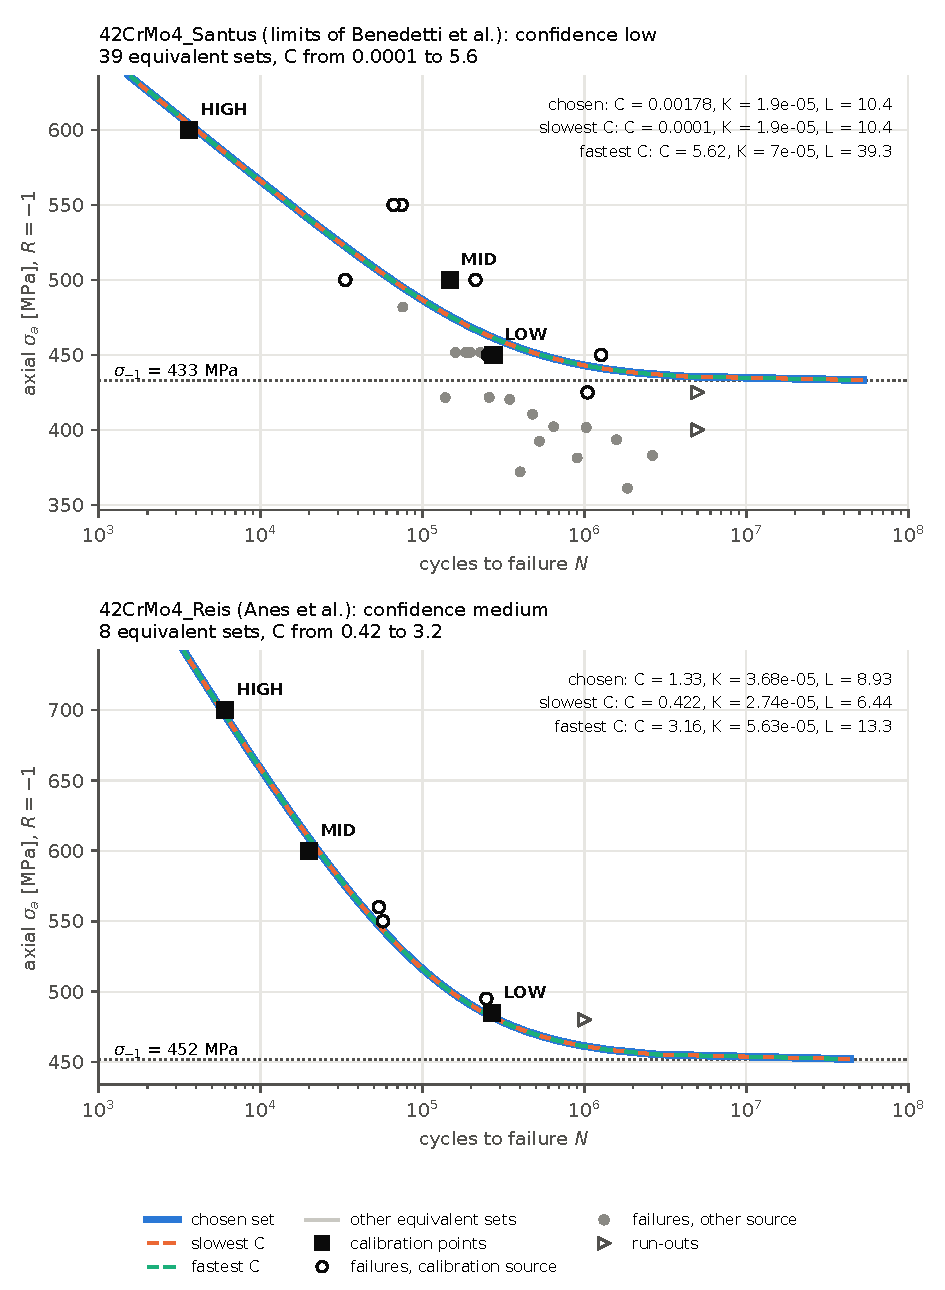
\includegraphics[width=0.85\textwidth]{fig_example_42CrMo4.pdf}
  \caption{Example 3, 42CrMo4. Top: the limit of Benedetti et al.\ lies above many failures of Santus et al.\
  (grey); the steep upper branch through the single HIGH point goes with $L\ge10$ in every equivalent set.
  Bottom: Anes et al., points spread
  over 485 to 700~MPa and $6\times10^3$ to $2.7\times10^5$ cycles.}
  \label{fig:cr}
\end{figure}

\begin{lesson}
A limit must agree with the failures of the database, not only with those of its own source: the Santus workbook
pools two sources under the limit of one, and the confidence flags it as major. The single HIGH specimen makes the
curve steep and forces a large $L$, which makes damage explode when $\beta$ is large; check such a point against
other data of the same batch before fitting. Points spread over a wide range of stress and life (the Reis workbook)
narrow $C$ to less than one decade, so the finding \code{C\_not\_identified} does not appear.
\end{lesson}

\FloatBarrier
%---------------------------------------------------------------------------------------------------------------------
\subsection*{Example 4: Al7075-T651 --- no inputs file, and a limit defined at $10^6$ cycles}
Data: Wang et al., \texttt{18\_Al7075\_T651\_Wang.xlsx}, calibrated as supplied, without an inputs file.
\begin{description}[leftmargin=0pt,font=\normalfont\bfseries]
\item[Step 1.] The source gives no measured limit; $\sigm=221.99$~MPa is its axial S--N curve at $10^6$ cycles, and
  $\taum=127.1$~MPa, so $\lambda=-1.9$~MPa.
\item[Step 2.] No material type is declared, so route 4: $A=221.99/561=0.3957$.
\item[Step 3.] Five failures; levels 235, 260 and 315~MPa above $\sigm$ (1, 2 and 1 specimens), so MID is 260~MPa.
  \begin{center}
  \begin{tabular}{@{}l l r r r@{}}
  \toprule
  Point & Specimen & $\sigma_a$ [MPa] & $N_\text{exp}$ & Residual \\
  \midrule
  LOW & AXIAL\_4 & 235.0 & 848\,760 & $-0.06$ / $-0.07$ \\
  MID & AXIAL\_3 & 260.0 & 159\,980 & $+0.06$ / $+0.05$ \\
  HIGH & AXIAL\_1 & 315.0 & 35\,094 & $-0.01$ / $-0.02$ \\
  \bottomrule
  \end{tabular}
  \end{center}
\item[Steps 4--5.] $\Emin=2.45\times10^{-4}$; 37 equivalent sets, $C$ from $10^{-4}$ to 3.16. Chosen: $C=1$,
  $K=1.40\times10^{-5}$, $L=6.66$ (Fig.~\ref{fig:wang}).
\item[Confidence.] Medium, five minor findings. One failure lies below $\sigm$, at 215~MPa, but after
  $1.19\times10^6$ cycles, that is after the reference life of the limit: it agrees with the limit, although the model
  predicts an infinite life for it. The others: $A$ estimated, Goodman because no material type is declared, $C$ not
  identified, single specimens.
\end{description}

\begin{figure}[ht]
  \centering
  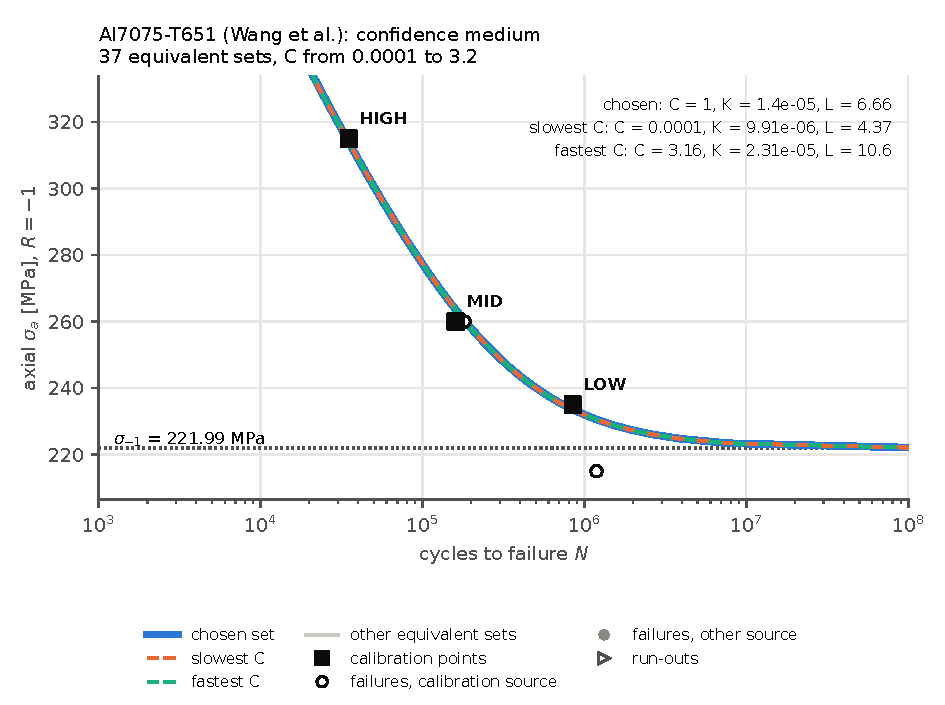
\includegraphics[width=0.85\textwidth]{fig_example_Al7075T651.pdf}
  \caption{Example 4, Al7075-T651. The failure at 215~MPa lies below $\sigm$, after the $10^6$ cycles at which
  $\sigm$ is defined.}
  \label{fig:wang}
\end{figure}

\begin{lesson}
A workbook alone is enough for a calibration; the findings then say what an inputs file would improve. For a
material without a true fatigue limit, a failure below the limit is judged at the life where the limit is defined:
before it, the data contradict the limit (major); after it, they agree with it (minor).
\end{lesson}

\FloatBarrier
%=====================================================================================================================
\section{Checklist}
%=====================================================================================================================
\begin{itemize}
\item Limits, $A$ and the three points come from the same source, or the difference is stated.
\item $\sigm$ is consistent with the run-outs and the failures near the limit, also those of other sources in the
  same database; the life at which $\sigm$ is defined is known.
\item The route to $A$ is the best one the data allow (1 before 2 before 3 and 4), and the $\Su$ used is recorded.
\item The three points follow the rule of Step 3; none is a lone specimen in conflict with other data; their stresses
  are well separated.
\item The whole family of equivalent sets is kept and checked with G1 and G2, from the lowest $E$ up.
\item The chosen set, the range of $C$ among the equivalent sets and the confidence are reported together.
\item All other tests are predicted with the transient model, and no constant is changed after seeing them.
\end{itemize}

\subsection*{Constants of the examples}
\begin{center}
\small
\begin{tabular}{@{}l r r r r r r l@{}}
\toprule
Workbook & $\sigm$ & $\taum$ & $A$ & $C$ & $K$ & $L$ & Confidence \\
\midrule
Al7075-T6 & 143.8 & 100.9 & 0.3584 & $1.00\times10^{-4}$ & $3.29\times10^{-6}$ & 2.97 & medium \\
Ti6Al4V, Berto & 475.74 & 388.25 & 0.4864 & $5.62\times10^{-4}$ & $7.70\times10^{-6}$ & 3.61 & medium \\
Ti6Al4V, Meneghetti & 500 & 422.5 & 0.5102 & 1.33 & $1.71\times10^{-4}$ & 0.05 & low \\
42CrMo4, Santus & 433 & 344 & 0.2063 & $1.78\times10^{-3}$ & $1.90\times10^{-5}$ & 10.4 & low \\
42CrMo4, Reis & 452 & 372 & 0.2850 & 1.33 & $3.68\times10^{-5}$ & 8.93 & medium \\
Al7075-T651, Wang & 221.99 & 127.1 & 0.3957 & 1.00 & $1.40\times10^{-5}$ & 6.66 & medium \\
\bottomrule
\end{tabular}
\end{center}

%=====================================================================================================================
\begin{thebibliography}{9}
\bibitem{tveit2025} S.~Tveit, N.~S.~Ottosen, E.~Erduran, A.~Reyes. Continuum mechanics fatigue model for arbitrary
  ratios of shear and normal stress fatigue strengths. \emph{Mechanics of Materials} 209 (2025) 105452.
\bibitem{ottosen2008} N.~S.~Ottosen, R.~Stenstr\"om, M.~Ristinmaa. Continuum approach to high-cycle fatigue
  modeling. \emph{International Journal of Fatigue} 30 (2008) 996--1006.
\bibitem{fkm} FKM Guideline: Analytical Strength Assessment of Components. Forschungskuratorium Maschinenbau (FKM),
  VDMA Verlag.
\end{thebibliography}

\end{document}
